\documentclass[tikz,border=3mm,multi=tikzpicture]{standalone}
\usepackage[utf8]{inputenc}
\usepackage[T1]{fontenc}
\usepackage{helvet}
\renewcommand{\familydefault}{\sfdefault}
\usepackage{tikz}
\usetikzlibrary{arrows.meta,positioning}
\begin{document}

\tikzset{every node/.append style={font=\sffamily\small}}

% TikZ 1
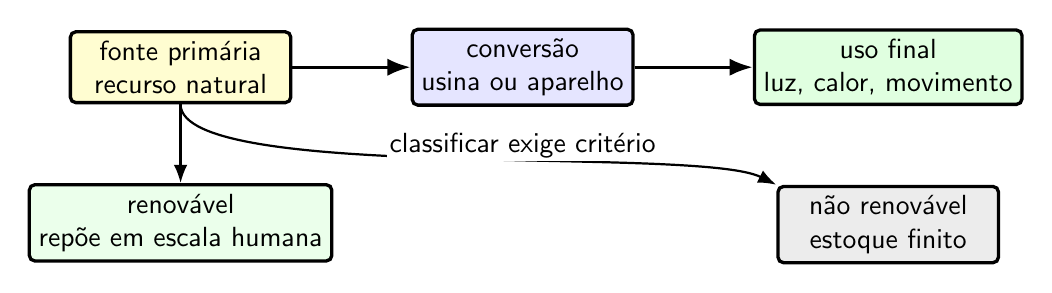
\begin{tikzpicture}[>=Latex,node distance=0.9cm]
  \tikzstyle{box}=[draw,rounded corners=2pt,minimum width=2.8cm,minimum height=0.9cm,align=center,very thick]
  \node[box,fill=yellow!18] (fonte) {fonte primária\\recurso natural};
  \node[box,fill=blue!10,right=1.5cm of fonte] (conv) {conversão\\usina ou aparelho};
  \node[box,fill=green!12,right=1.5cm of conv] (uso) {uso final\\luz, calor, movimento};
  \draw[very thick,->] (fonte) -- (conv);
  \draw[very thick,->] (conv) -- (uso);
  \node[box,fill=green!8,below=1.0cm of fonte] (ren) {renovável\\repõe em escala humana};
  \node[box,fill=gray!15,below=1.0cm of uso] (naoren) {não renovável\\estoque finito};
  \draw[thick,->] (fonte.south) -- (ren.north);
  \draw[thick,->] (fonte.south) .. controls +(0,-1.0) and +(-1.0,0.5) .. (naoren.north west);
  \node[align=center,fill=white,inner sep=1pt,below=0.3cm of conv] {classificar exige critério};
\end{tikzpicture}

% TikZ 2
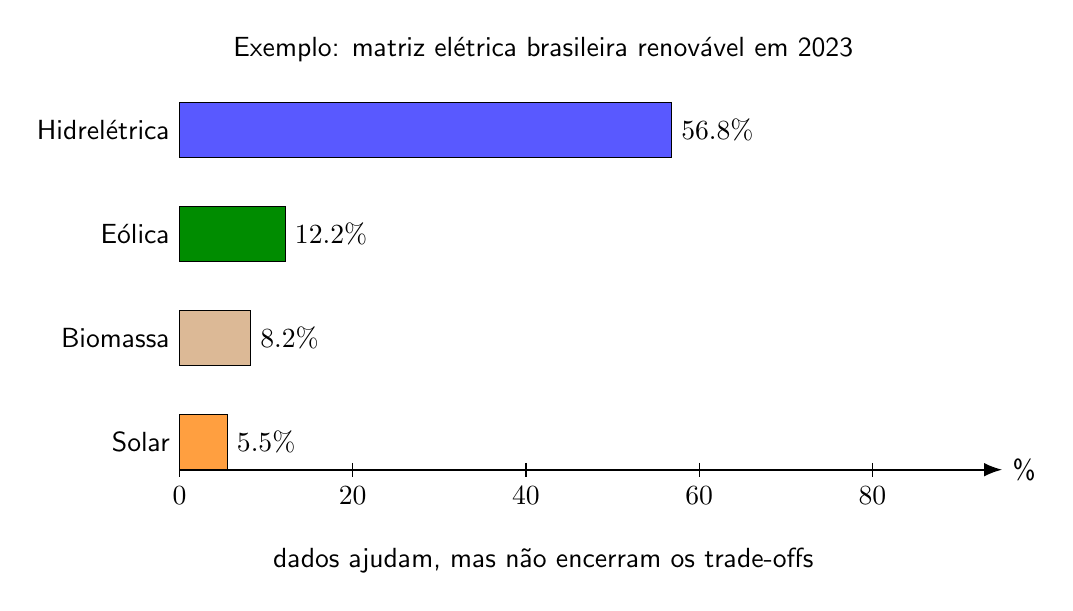
\begin{tikzpicture}[x=0.11cm,y=0.22cm,>=Latex]
  \draw[->,thick] (0,0) -- (95,0) node[right] {\%};
  \foreach \x in {0,20,40,60,80}{
    \draw (\x,0.4) -- (\x,-0.4);
    \node[below] at (\x,-0.4) {$\x$};
  }
  \foreach \y/\name/\value/\color in {
    18/Hidrelétrica/56.8/blue!65,
    12/Eólica/12.2/green!55!black,
    6/Biomassa/8.2/brown!55,
    0/Solar/5.5/orange!75
  }{
    \draw[fill=\color] (0,\y) rectangle (\value,\y+3.2);
    \node[left] at (0,\y+1.6) {\name};
    \node[right] at (\value,\y+1.6) {$\value\%$};
  }
  \node[align=center,above] at (42,23) {Exemplo: matriz elétrica brasileira renovável em 2023};
  \node[align=center,below] at (42,-4) {dados ajudam, mas não encerram os trade-offs};
\end{tikzpicture}

\end{document}
